\section{Parser}

In our recursive-descent Parser we implemented all EBNF production rules as
methods. The production rules of our EBNF allows alternatives, repetitions and optional parts.
Figure (\ref{parser_deb}) shows a dependence diagram of the parser methods.  

To ensure that our EBNF is LL(1) conform, we created the a list with the first sets.
The parser compares the actual token with the first-sets symbol
and takes decisions between alternatives. 
To guarantee that the decision between two alternatives is correct, the first
set of the alternatives must be disjunctive. We checked our EBNF with the Parser tool: coco, to ensure we are are LL(1) conform.
% coco page http://www.ssw.uni-linz.ac.at/Research/Projects/Coco/

\begin{figure}[h]
\label{parser_deb}
\begin{center}
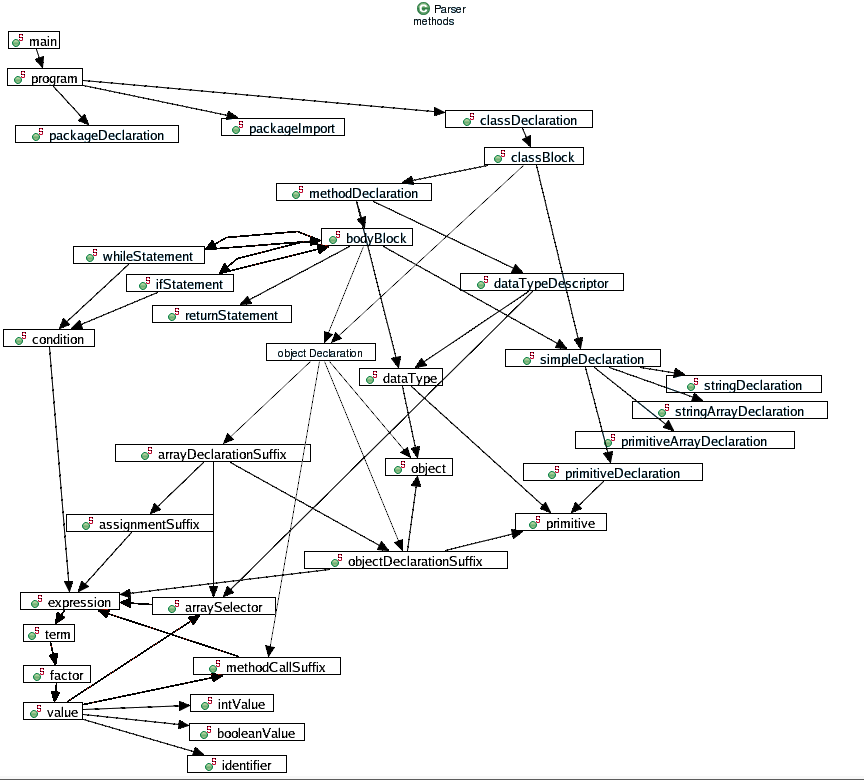
\includegraphics[width=13cm,height=13cm]{images/parser_edit.png}
\end{center}
\caption{parser methods dependencies}
\end{figure}


\subsection{First Symbols(first sets)}
\label{first_sets}
\noindent
\begin{tabularx}{\linewidth}{YY}
program & ``\texttt{package}'' ``\texttt{import}'' ``\texttt{public}'' \\
packageDeclaration & ``\texttt{package}'' \\
packageImport & ``\texttt{import}'' \\
classDeclaration & ``\texttt{public}'' \\
identifier & simpleIdentifier \\
classBlock & simpleIdentifier ``\texttt{public}'' ``\texttt{String}'' ``\texttt{String[]}'' ``\texttt{int}'' ``\texttt{boolean}'' ``\texttt{char}'' ``\texttt{int[]}'' ``\texttt{boolean[]}'' ``\texttt{char[]}'' \\
objectDeclaration & simpleIdentifier \\
simpleDeclaration & ``\texttt{String}'' ``\texttt{String[]}'' ``\texttt{int}'' ``\texttt{boolean}'' ``\texttt{char}'' ``\texttt{int[]}'' ``\texttt{boolean[]}'' ``\texttt{char[]}'' \\
methodDeclaration & ``\texttt{public}'' \\
object & simpleIdentifier \\
objectDeclarationSuffix & simpleIdentifier \\
primitiveDeclaration & ``\texttt{int}'' ``\texttt{boolean}'' ``\texttt{char}'' \\
primitiveArrayDeclaration & ``\texttt{int[]}'' ``\texttt{boolean[]}'' ``\texttt{char[]}'' \\
stringDeclaration & ``\texttt{String}'' \\
stringArrayDeclaration & "String[]" \\
datatype & simpleIdentifier "String" "int" "boolean" "char" \\
datatypeDescriptor & simpleIdentifier "String" "int" "boolean" "char" \\
bodyBlock & simpleIdentifier "String" "String[]" "while" "if" "return" "int" "boolean" "char" "int[]" "boolean[]" "char[]" \\
primitive & "int" "boolean" "char" \\
assignmentSuffix & equal \\
primitiveArray & "int[]" "boolean[]" "char[]" \\
objectDeclarationAssignmentMethodcall & simpleIdentifier \\
arrayDeclarationSuffix & equal simpleIdentifier "[" \\
methodCallSuffix & "(" \\
expression & not number simpleIdentifier StringValue charValue "NULL" "-" "true" "false" \\
arraySelector & "[" \\
whileStatement & "while" \\
ifStatement & "if" \\
returnStatement & "return" \\
condition & not number simpleIdentifier StringValue charValue "NULL" "-" "true" "false" \\
value & not number simpleIdentifier StringValue charValue "NULL" "-" "true" "false" \\
intValue & number "-" \\
booleanValue & "true" "false" \\
factor & not number simpleIdentifier StringValue charValue "NULL" "-" "true" "false" \\
term & not number simpleIdentifier StringValue charValue "NULL" "-" "true" "false" \\
\end{tabularx}
%

\newpage
\section{Syntax Error Handling}
The Compiler is able to detect a certain amount of Syntax Errors. We distinguish between two error levels : week and strong errors.
\begin{itemize}
  \item \textbf{Week Errors} will be fixed by the parser. 
  \item \textbf{Strong Errors} can not be fixed. 
\end{itemize}

\subsection{Week Errors (Warnings)}
\label{label_week_errors}
Week errors are missing tokens which will be inserted by the parser.
The code generator never get notice about those errors. When a week error occurs a warning will be displaced, the token will be
inserted, parsing and code generation continues.
Compiler is able to detect and correct following week errors:
\begin{itemize}
  \item any missing ";"
  \item any missing ")" "\{" "\}" "]" 
  \item near all missing "(" except in an object declaration, because we have to distinguish between "[" and "(" 
  \item in class declarations a missing ``class'' will be fixed.
  \item in method declarations when return type is missing (TODO !!!)
  \item in method declarations when ``static'' is missing
  \item in parameterlists we will detect and correct missing ","
\end{itemize}

\subsection{Strong Errors}
\label{label_strong_errors}
Strong Errors can be syntax errors as well as invalid symbols or invalid words. When a strong error occurs the parser displaces a error
message and the code generation will be stopped. The parser goes to the next strong symbol and continue parsing. In our parser
implementation we have sync operation implemented in three methods. See Figure (\ref{parser_deb}), marked methods (TODO) serves as
synchronisation points. Synchronization works this way:
\begin{itemize}
  \item one of the synchronization methods recognizes a strong error in one of its called method
  \item the error will be printed and code generation will stop
  \item the synchronization methods x fetches new tokens until the next ``\hyperref[first_sets]{first set}'' token of method x is fetched
\end{itemize}
Strong Errors can be:
\begin{itemize}
  \item misplaced tokens. When the current token does not correspond to EBNF rules, except of week errors.
  \item any missing identifiers.
  \item any illegal terminal symbols, like identifier starting with a digit. This kind of error detects the scanner, and a
  error token will be delivered to the parser.
\end{itemize}
\begin{quote}
For example, if we had a production
\begin{verbatim}
A = a b c.
\end{verbatim}
for which the input was
\begin{verbatim}
a x c
\end{verbatim}
the parser reports
\begin{verbatim}
TODO Message
\end{verbatim}
\end{quote}


\section{Symboltable}

The Parser produces for every field (global variables, methods) and local variables an entry in the Symboltable.
The Symboltable is implemented as a Java Linked List. We distinguish between different scopes. The global scope and local scopes. Every
method declaration has an entry in the gobal scope. The method's variables (local vars)  are not in the same list (global scope), they are in
a separate linked list which is an attribute of the methode. TODO FIGURE

The Symboltable is representet by the symboltable list (SymbolTableList.java) which consists of cells (SymbolTableCell.java).
A cell consists of:
\newline
\newline
\begin{tabular}{lp{6cm}}
\texttt{String name} & Name of the entry (Variable name, Method name,\ldots) \\
\texttt{ClassType classType} & kind of the entry: variable, array, procedure \\
\texttt{TypeDesc type} & data type: int, bool, char, String \\
\texttt{String value} & the value of the variable, when available \\
\texttt{SymbolTableList methodSymbols} & only methods and arrays have a sub list with symbol table cells \\
\texttt{int offset} & offset is negative \\
\texttt{int size} & in 4 bytes (word) \\
\end{tabular}


\section {Type Savety}

\subsection{Naming convention}
We ensure that variable names in a separate scope are unique. Local variables can have the same name as global variables. 

\subsection{Operator on incompatible Types}
\begin{itemize}
  \item will be ensured by EBNF
  \item 
\end{itemize}

\subsection{Typechecking}




